% !TeX TS-program = XeLaTeX
% ارائه دفاع پایان‌نامه — PDF فارسی (هر صفحه = یک اسلاید)
% کامپایل از همین پوشه:
%   xelatex defense_fa.tex && xelatex defense_fa.tex
\documentclass[10pt]{article}

\usepackage[
  paperwidth=297mm,
  paperheight=167mm,
  margin=10mm,
  top=9mm,
  bottom=12mm
]{geometry}
% سازگاری bidi/xepersian با tabular در LaTeX جدید
\makeatletter
\providecommand{\UseMathForPositioningText}{}
\providecommand{\@kernel@tabular@init}{}
\makeatother
\usepackage{graphicx}
\usepackage{amsmath,amssymb}
\usepackage{booktabs}
\usepackage{array}
\usepackage[table]{xcolor}
\usepackage{colortbl}
\usepackage{tikz}
\usepackage{fancyhdr}
\usepackage{hyperref}

\graphicspath{{../img/}}
\pagestyle{fancy}
\fancyhf{}
\renewcommand{\headrulewidth}{0pt}
\renewcommand{\footrulewidth}{0.4pt}
% در سند RTL، سمت راست بصری = شروع خط فارسی
\fancyfoot[R]{\small\color{UTmuted}\thepage}
\fancyfoot[L]{\small\color{UTmuted}دفاع کارشناسی ارشد — دانشگاه تهران}

\setlength{\itemsep}{0.2em}
\setlength{\parsep}{0pt}
\setlength{\topsep}{0.25em}

\definecolor{UTnavy}{HTML}{0B2C4A}
\definecolor{UTteal}{HTML}{1A6B6B}
\definecolor{UTgold}{HTML}{C47A2C}
\definecolor{UTsoft}{HTML}{E8EEF2}
\definecolor{UTmuted}{HTML}{4A5563}
\definecolor{UTcard}{HTML}{F7FAFC}

\newcommand{\slidetitle}[1]{%
  \vspace*{-2mm}%
  {\LARGE\color{UTnavy}\textbf{#1}}\par
  \vspace{1mm}%
  {\color{UTgold}\rule{35mm}{1.2pt}}\par
  \vspace{3mm}%
}
\newcommand{\newslide}{\clearpage}
% جعبه‌ها با minipage؛ در XePersian با \raggedright متن به راست می‌چسبد
\newcommand{\cardbox}[2]{%
  \fcolorbox{UTsoft}{UTcard}{%
    \begin{minipage}[t]{#1}
      \raggedright
      #2
    \end{minipage}%
  }%
}
\newcommand{\keybox}[1]{%
  \noindent
  \fcolorbox{UTteal}{UTsoft}{%
    \begin{minipage}{0.96\textwidth}
      \raggedright
      #1
    \end{minipage}%
  }\par
}
\newcommand{\warnbox}[1]{%
  \noindent
  \fcolorbox{UTgold}{UTsoft}{%
    \begin{minipage}{0.96\textwidth}
      \raggedright
      #1
    \end{minipage}%
  }\par
}

\usepackage{fontspec}
\usepackage{xepersian}
\settextfont[Path={../font/},
  BoldFont={IRLotusICEE_Bold.ttf},
  BoldItalicFont={IRLotusICEE_BoldIranic.ttf},
  ItalicFont={IRLotusICEE_Iranic.ttf},
  Scale=0.92]{IRLotusICEE.ttf}
\setdigitfont[Path={../font/}, Scale=0.92]{IRLotusICEE.ttf}
\setlatintextfont[Path={../font/},
  BoldFont={LiberationSerif-Bold.ttf},
  ItalicFont={LiberationSerif-Italic.ttf},
  BoldItalicFont={LiberationSerif-BoldItalic.ttf},
  Scale=0.88]{LiberationSerif-Regular.ttf}

\hypersetup{
  pdftitle={دفاع پایان‌نامه: طراحی و بهینه‌سازی الگوریتم اجماع مقیاس‌پذیر},
  pdfauthor={سجاد خشدونی فراهانی},
  colorlinks=true,
  linkcolor=UTnavy,
  urlcolor=UTteal
}

\begin{document}

%================ TITLE ================
\thispagestyle{empty}
\begin{tikzpicture}[remember picture,overlay]
  \fill[UTnavy] (current page.south west) rectangle (current page.north east);
  \fill[UTgold] ([yshift=-48mm]current page.north west) rectangle ([yshift=-49.2mm]current page.north east);
\end{tikzpicture}
\vspace*{12mm}
\begin{center}
{\large\textcolor{UTsoft}{دانشگاه تهران — پردیس دانشکده‌های فنی}}\\[2mm]
{\normalsize\textcolor{UTsoft}{دانشکده علوم مهندسی | گروه الگوریتم‌ها و محاسبات}}\\[10mm]
{\Huge\textbf{\textcolor{white}{طراحی و بهینه‌سازی الگوریتم اجماع مقیاس‌پذیر}}}\\[3mm]
{\Huge\textbf{\textcolor{white}{برای سیستم‌های بلاکچین}}}\\[8mm]
{\Large\textcolor{UTgold}{جلسه دفاع پایان‌نامه کارشناسی ارشد — مهندسی کامپیوتر}}\\[12mm]
\begin{tabular}{ccc}
\textcolor{UTgold}{دانشجو} & \textcolor{UTgold}{استاد راهنما} & \textcolor{UTgold}{تاریخ} \\[1mm]
\textbf{\textcolor{white}{سجاد خشدونی فراهانی}} &
\textbf{\textcolor{white}{دکتر علی کمندی}} &
\textbf{\textcolor{white}{فروردین ۱۴۰۵}}
\end{tabular}
\end{center}

%================ OUTLINE ================
\newslide
\slidetitle{ساختار ارائه}
\begin{enumerate}
  \item مقدمه و ضرورت مقیاس‌پذیری بلاکچین
  \item بیان مسئله، گلوگاه‌ها و سه‌گانه بلاکچین
  \item اهداف، پرسش‌ها و دامنه پژوهش
  \item مرور راهکارهای موجود و جایگاه پژوهش
  \item معماری پیشنهادی: زنجیره اصلی + زنجیره‌های جانبی
  \item تابع تخصیص قطعی، الگوریتم پردازش و نهایی‌سازی
  \item مدل ریاضی توان عملیاتی و مقیاس‌پذیری افقی
  \item نتایج آزمایش‌ها، بنچمارک \lr{Rust} و تفکیک روش‌شناختی
  \item امنیت، دستاوردها، محدودیت‌ها و کارهای آینده
\end{enumerate}

%================ INTRO ================
\newslide
\slidetitle{مقدمه: چرا مقیاس‌پذیری؟}
\begin{itemize}
  \item بلاکچین با ترکیب رمزنگاری، شبکه همتا‌به‌همتا و اجماع، دفترکل مشترک بدون متولی مرکزی می‌سازد.
  \item بیتکوین نمونه پایدار این رویکرد است؛ اما معماری تک‌زنجیره‌ای ظرفیت را محدود می‌کند.
  \item در زنجیره عمومی کاملاً تکرارشونده، هر نود کامل تقریباً همه تراکنش‌ها را دریافت، ذخیره و اعتبارسنجی می‌کند.
  \item افزودن نود جدید برخلاف سامانه‌های توزیع‌شده متعارف، ظرفیت را افزایش نمی‌دهد؛ فقط افزونگی را بالا می‌برد.
  \item با افزایش تقاضا: استخر تراکنش پر می‌شود، کارمزد بالا می‌رود، و کاربردهایی مانند پرداخت خرد و امور مالی غیرمتمرکز آسیب می‌بینند.
\end{itemize}
\vspace{2mm}
\keybox{\textbf{پرسش محوری:} چگونه توان عملیاتی شبکه را افزایش دهیم، بدون آنکه امنیت زنجیره اصلی و اصل غیرمتمرکز بودن به‌طور جدی قربانی شود؟\\[1mm]
\textbf{پاسخ پیشنهادی:} معماری چندزنجیره‌ای؛ زنجیره اصلی به‌عنوان مرجع امنیتی و زنجیره‌های جانبی برای پردازش موازی.}

%================ PROBLEM ================
\newslide
\slidetitle{بیان مسئله: سه گلوگاه فنی}
\noindent
\begin{minipage}[t]{0.32\textwidth}
\cardbox{0.92\linewidth}{%
\textbf{\textcolor{UTteal}{گلوگاه یک: انتشار شبکه}}\\[1mm]
{\footnotesize
بلوک به اندازه \(B\) باید سریع به اکثریت نودها برسد.\\[0.8mm]
رابطه تقریبی: \(p_{fork}\approx 1-e^{-\Delta/T}\)\\[0.8mm]
اگر \(T\) کم یا \(B\) زیاد شود، نسبت \(\Delta/T\) بزرگ و فورک بیشتر می‌شود.}}
\end{minipage}\hfill
\begin{minipage}[t]{0.32\textwidth}
\cardbox{0.92\linewidth}{%
\textbf{\textcolor{UTteal}{گلوگاه دو: اعتبارسنجی}}\\[1mm]
{\footnotesize
هر امضای دیجیتال هزینه پردازنده دارد.\\[0.8mm]
تراکنش چندورودی چند بار این هزینه را تحمیل می‌کند.\\[0.8mm]
در نرخ بالا، پردازنده نود معمولی اشباع می‌شود.}}
\end{minipage}\hfill
\begin{minipage}[t]{0.32\textwidth}
\cardbox{0.92\linewidth}{%
\textbf{\textcolor{UTteal}{گلوگاه سه: وضعیت خروجی‌ها}}\\[1mm]
{\footnotesize
دسترسی تصادفی به مجموعه خروجی‌های خرج‌نشده.\\[0.8mm]
با رشد نرخ تراکنش، دیسک و حافظه نهان محدود می‌شوند.\\[0.8mm]
ظرفیت کل تقریباً برابر کندترین نود قابل‌قبول است.}}
\end{minipage}

\vspace{2mm}
\keybox{\textbf{معنی پارامترها}\\[1mm]
{\footnotesize
\(B\) = اندازه بلوک \hfill
\(\Delta\) = تأخیر مؤثر انتشار بلوک در شبکه \hfill
\(T\) = فاصله متوسط تولید بلوک \hfill
\(p_{fork}\) = احتمال فورک موقت\\[1mm]
در بیتکوین معمولاً \(T\approx 600\) ثانیه و \(B\) حدود یک مگابایت است؛ بنابراین نمی‌توان \(T\) را آزادانه خیلی کوچک کرد.}}

\vspace{1.5mm}
\warnbox{\textbf{صورت‌بندی طراحی مقید}\\[0.5mm]
{\footnotesize
هدف: بیشینه‌کردن \(TPS\) با این قیدها:\\[0.5mm]
امنیت نزدیک به زنجیره اصلی \(C_0\)؛
هزینه هر نود متناسب با \(TPS/N\)؛
تابع تخصیص \(A\) قطعی و عمومی؛
احتمال دوبارخرج تقریباً مانند بیتکوین.}}

%================ TRILEMMA ================
\newslide
\slidetitle{سه‌گانه بلاکچین و رویکرد پژوهش}
\noindent
\begin{minipage}[t]{0.42\textwidth}
\cardbox{0.92\linewidth}{%
\textbf{\color{UTteal}سه‌گانه (\lr{Trilemma})}\\[2mm]
\begin{enumerate}
  \item مقیاس‌پذیری
  \item امنیت
  \item غیرمتمرکز بودن
\end{enumerate}
\vspace{1mm}
در بیتکوین، امنیت و تمرکززدایی بر ظرفیت ترجیح داده شده‌اند (فاصله بلوک طولانی + محدودیت اندازه).}
\end{minipage}\hfill
\begin{minipage}[t]{0.54\textwidth}
\cardbox{0.92\linewidth}{%
\textbf{\color{UTteal}رویکرد این پایان‌نامه}\\[2mm]
حذف کامل سه‌گانه ادعا نمی‌شود.\\[1mm]
به‌جای آن: \textbf{جداسازی نقش‌ها}\\[1mm]
\begin{itemize}
  \item زنجیره اصلی = مرجع امنیتی و قطعیت نهایی
  \item زنجیره‌های جانبی = پردازش موازی تراکنش
  \item فشار تراکنشی از لایه امنیتی جدا می‌شود
  \item مقیاس‌پذیری از نوع \textbf{افقی} است، نه صرفاً عمودی
\end{itemize}}
\end{minipage}

\vspace{4mm}
از دید صف: یک صف مرکزی با ظرفیت محدود به چند صف موازی تبدیل می‌شود. اگر بار متعادل باشد، نرخ خروج کل ≈ مجموع نرخ خروج زنجیره‌های جانبی.

%================ GOALS ================
\newslide
\slidetitle{اهداف پژوهش}
\begin{enumerate}
  \item ارائه معماری چندزنجیره‌ای مبتنی بر زنجیره اصلی و چند زنجیره جانبی موازی
  \item تعریف تابع تخصیص قطعی برای نگاشت \lr{UTXO}/تراکنش به زنجیره‌های جانبی
  \item حفظ نقش امنیتی زنجیره اصلی از طریق ثبت ارجاع رمزنگاری‌شده بلوک‌های جانبی
  \item کاهش تأخیر تأیید اولیه با فاصله بلوک کوتاه‌تر در زنجیره‌های جانبی، حدود یک دقیقه
  \item تحلیل تئوری مقیاس‌پذیری افقی و رابطه \(TPS\) با تعداد زنجیره‌ها \(N\)
  \item پیاده‌سازی نمونه اولیه در زبان \lr{Rust} و ارزیابی تفکیک‌شده از مدل شبکه
  \item شناسایی محدودیت‌ها، ریسک‌های امنیتی و مسیر توسعه آینده
\end{enumerate}

%================ QUESTIONS ================
\newslide
\slidetitle{پرسش‌های پژوهش و دامنه}
\keybox{\textbf{پرسش‌ها}\\[1mm]
\begin{enumerate}
  \item چگونه تراکنش‌ها را تقسیم کنیم بدون افزایش غیرقابل‌کنترل دوبارخرج؟
  \item نقش زنجیره اصلی به‌عنوان مرجع امنیتی چیست؟
  \item رابطه تعداد زنجیره‌های جانبی با توان عملیاتی کل چگونه است؟
  \item تفاوت توان نظری شبکه و بنچمارک محاسباتی پیاده‌سازی چیست؟
  \item مهم‌ترین ریسک‌های امنیتی، مهندسی و عملیاتی کدام‌اند؟
\end{enumerate}}
\vspace{3mm}
\warnbox{\textbf{دامنه و فرضیات:} تمرکز بر بلاکچین‌های مبتنی بر مدل \lr{UTXO}؛ زنجیره اصلی با اثبات کار و قاعده بیشترین کار انباشته؛ تخصیص قطعی و عمومی؛ نمونه اولیه برای ارزیابی معماری است و جایگزین شبکه تولیدی عمومی نیست.}

%================ TAXONOMY ================
\newslide
\slidetitle{تکسونومی روش‌های مقیاس‌پذیری}
\begin{center}
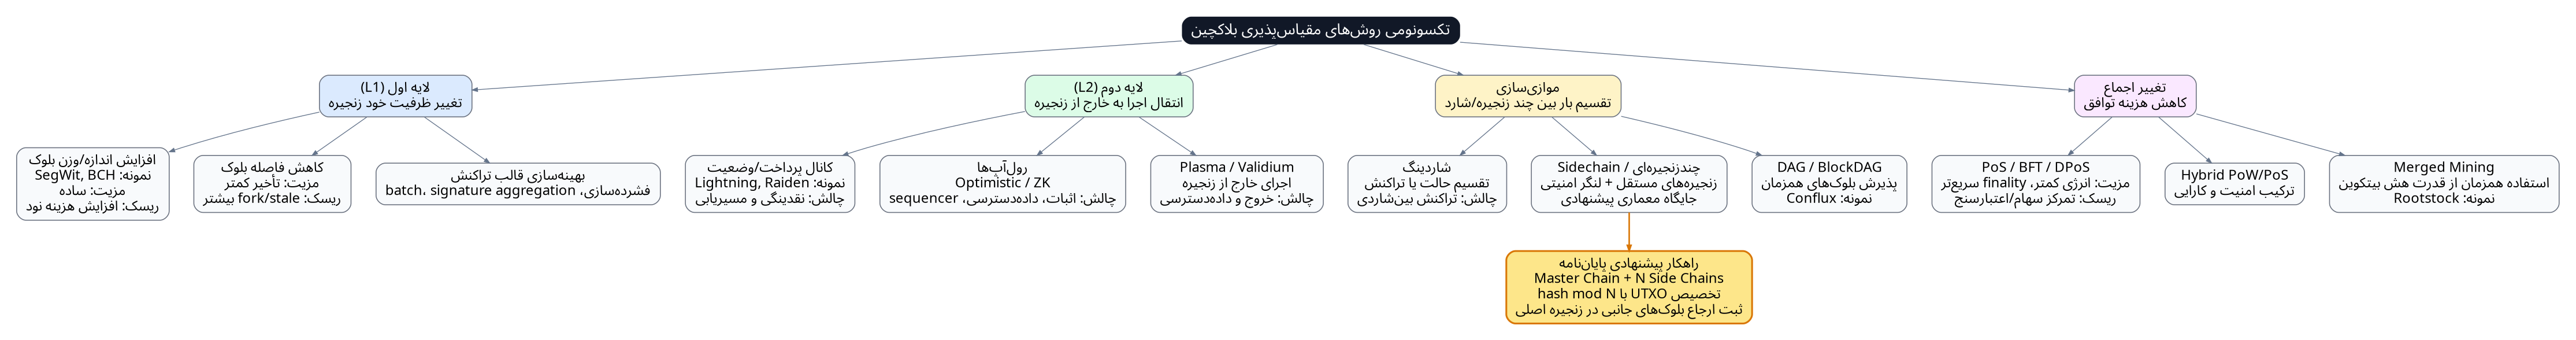
\includegraphics[width=0.95\textwidth,height=0.78\textheight,keepaspectratio]{taxonomy_blockchain_scaling.png}
\end{center}

%================ COMPARISON ================
\newslide
\slidetitle{مقایسه کیفی راهکارهای موجود}
\begin{center}
\renewcommand{\arraystretch}{1.25}
\small
\begin{tabular}{>{\raggedleft\arraybackslash}p{2.6cm}>{\raggedleft\arraybackslash}p{2.8cm}>{\raggedleft\arraybackslash}p{2.6cm}>{\raggedleft\arraybackslash}p{4.2cm}}
\toprule
\textbf{راهکار} & \textbf{نقطه قوت} & \textbf{رشد ظرفیت} & \textbf{محدودیت اصلی} \\
\midrule
بیتکوین پایه & امنیت بسیار بالا & ثابت & اندازه و زمان بلوک \\
افزایش اندازه بلوک & سادگی لایه اول & محدود & تمرکز نود / هزینه سخت‌افزار \\
لایتنینگ & مناسب پرداخت خرد & وابسته به نقدینگی & مسیریابی و مدیریت کانال \\
رول‌آپ & نزدیک امنیت لایه ۱ & بالا & داده‌دسترسی و \lr{Sequencer} \\
شاردینگ & موازی‌سازی حالت & تقریباً خطی & امنیت شارد و تراکنش بین‌شاردی \\
زنجیره جانبی کلاسیک & انعطاف‌پذیر & متغیر & مدل اعتماد پل \\
\rowcolor{UTsoft}
\textbf{معماری پیشنهادی} & مرجع PoW + موازی & تقریباً خطی با \(N\) & بین‌زنجیره‌ای و هماهنگی \\
\bottomrule
\end{tabular}
\end{center}
\vspace{3mm}
\keybox{\textbf{جایگاه پژوهش:} ترکیب مزایای زنجیره اصلی امن با پردازش موازی زنجیره‌های جانبی، در مدل سازگار با \lr{UTXO} و با تابع تخصیص قطعی.}

%================ ARCHITECTURE ================
\newslide
\slidetitle{نمای کلی معماری پیشنهادی}
\begin{center}
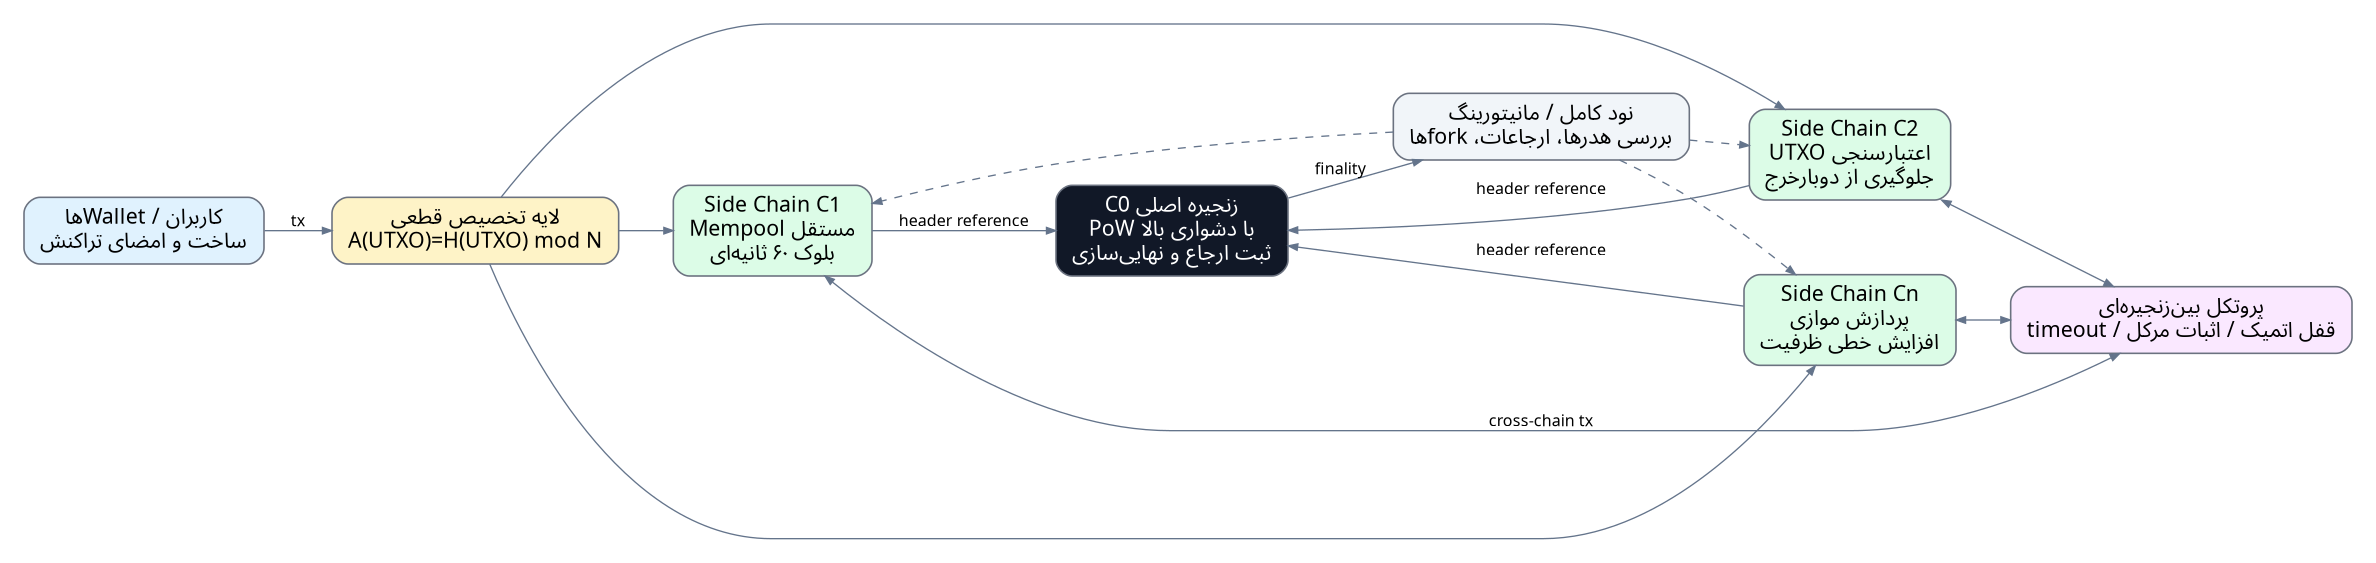
\includegraphics[width=0.92\textwidth,height=0.62\textheight,keepaspectratio]{architecture_master_sidechain.png}
\end{center}
\vspace{1mm}
{\small جریان کار: کاربر → تابع تخصیص → استخر زنجیره جانبی → بلوک جانبی → ارجاع در زنجیره اصلی → نهایی‌سازی پس از \(k\) تأیید}

%================ SYSTEM MODEL ================
\newslide
\slidetitle{مدل سیستم و نقش زنجیره‌ها}
\keybox{\textbf{تعریف رسمی}\\[1mm]
\[
\mathcal{S}=\langle P,\, C_0,\, \{C_i\}_{i=1}^{N},\, U,\, M,\, A,\, R\rangle
\]
\(P\) نودها/ماینرها؛ \(C_0\) زنجیره اصلی؛ \(C_i\) زنجیره‌های جانبی؛ \(U\) مجموعه \lr{UTXO}؛ \(M\) استخرها؛ \(A\) تابع تخصیص؛ \(R\) ارجاعات ثبت‌شده در \(C_0\).}

\vspace{3mm}
\noindent
\begin{minipage}[t]{0.48\textwidth}
\cardbox{0.92\linewidth}{%
\textbf{\color{UTteal}زنجیره اصلی \(C_0\)}\\[1mm]
\begin{itemize}
  \item اجماع: اثبات کار (\lr{PoW})
  \item فاصله بلوک \(\approx ۱۰\) دقیقه
  \item ثبت ارجاع بلوک‌های جانبی
  \item ترتیب نهایی و قطعیت اقتصادی
  \item مرجع فورک و بازسازماندهی
\end{itemize}}
\end{minipage}\hfill
\begin{minipage}[t]{0.48\textwidth}
\cardbox{0.92\linewidth}{%
\textbf{\color{UTteal}زنجیره جانبی \(C_i\)}\\[1mm]
\begin{itemize}
  \item فقط تراکنش‌های تخصیص‌یافته
  \item فاصله بلوک \(\approx ۱\) دقیقه
  \item تأیید اولیه سریع‌تر
  \item استخر و وضعیت محلی مستقل
  \item اتصال با \lr{parent\_master\_hash}
\end{itemize}}
\end{minipage}

%================ BLOCK STRUCTURE ================
\newslide
\slidetitle{ساختار بلوک و ارتباط زنجیره‌ها}
\noindent
\begin{minipage}[t]{0.48\textwidth}
\cardbox{0.92\linewidth}{%
\textbf{\color{UTteal}MasterBlock}\\[1mm]
{\small\lr{index, timestamp, references, previous\_hash, merkle\_root, nonce, difficulty}}\\[1mm]
هر ارجاع: شناسه زنجیره، ارتفاع، هش بلوک جانبی، ریشه مرکل تراکنش‌ها.}
\end{minipage}\hfill
\begin{minipage}[t]{0.48\textwidth}
\cardbox{0.92\linewidth}{%
\textbf{\color{UTteal}SideBlock}\\[1mm]
{\small\lr{index, side\_chain\_id, timestamp, transactions, previous\_hash, parent\_master\_hash, merkle\_root, nonce}}}
\end{minipage}
\vspace{3mm}
\begin{center}
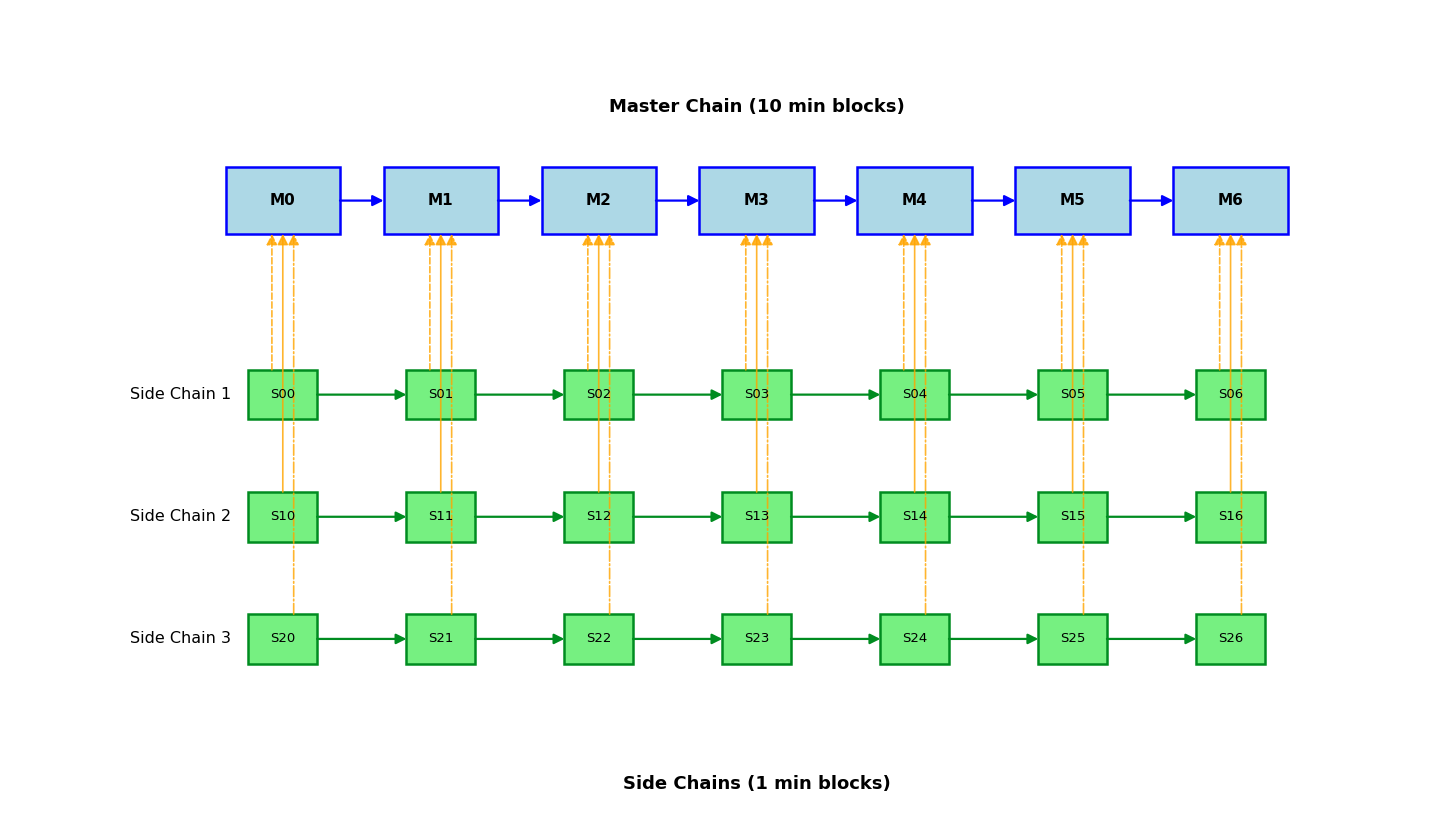
\includegraphics[width=0.78\textwidth,height=0.42\textheight,keepaspectratio]{chain_chart_all_sxy_to_my.png}
\end{center}

%================ ASSIGNMENT ================
\newslide
\slidetitle{تابع تخصیص قطعی}
\keybox{\textbf{ایده کلیدی}\\[1mm]
\[
A(utxo)=H(utxo)\bmod N
\]
\(H\): تابع هش رمزنگاری (مثلاً \lr{SHA-256})؛ \(N\): تعداد زنجیره‌های جانبی.}
\vspace{2mm}
\begin{itemize}
  \item همه نودها \textbf{بدون هماهنگ‌کننده مرکزی} همان زنجیره را محاسبه می‌کنند.
  \item هر خروجی خرج‌نشده فقط در یک قلمرو اعتبارسنجی خرج می‌شود → کنترل دوبارخرج در سطح تخصیص.
  \item توزیع شبه‌تصادفی هش به تعادل بار کمک می‌کند (در فرض توزیع مناسب خروجی‌ها).
  \item در تراکنش چندورودی: اگر همه ورودی‌ها هم‌قلمروی باشند، تک‌زنجیره‌ای است؛ وگرنه بین‌زنجیره‌ای.
\end{itemize}
\vspace{2mm}
\warnbox{\textbf{نکته مهندسی:} تغییر \(N\) مقدار \(\bmod N\) را جابه‌جا می‌کند. افزودن/حذف زنجیره نیازمند سیاست \lr{Epoch}/مهاجرت یا درهم‌سازی سازگار است. در نسخه اولیه، \(N\) در هر دوره ثابت فرض می‌شود.}

%================ ALGORITHM ================
\newslide
\slidetitle{الگوریتم پردازش تراکنش}
\begin{enumerate}
  \item کاربر تراکنش را ایجاد و با امضای دیجیتال تأیید می‌کند.
  \item ورودی اصلی (یا مجموعه ورودی‌ها) با تابع تخصیص به زنجیره جانبی نگاشت می‌شود.
  \item تراکنش به استخر همان زنجیره ارسال می‌شود.
  \item نودها صحت امضا، وجود \lr{UTXO} و عدم دوبارخرج را بررسی می‌کنند.
  \item تولیدکننده بلوک، تراکنش‌های معتبر را در بلوک جانبی قرار می‌دهد.
  \item هش/هدر بلوک جانبی به زنجیره اصلی ارسال و در ارجاعات ثبت می‌شود.
  \item پس از \(k\) تأیید روی زنجیره اصلی، تراکنش نهایی تلقی می‌شود.
\end{enumerate}
\vspace{2mm}
\keybox{\textbf{شبه‌کد تخصیص}\\[1mm]
\begin{latin}\ttfamily\small
AssignTransaction(tx, N):\\
\quad u = SelectPrimaryInput(tx.inputs)\\
\quad h = SHA256(u.txid || u.index)\\
\quad return h mod N
\end{latin}}

%================ CROSS-CHAIN ================
\newslide
\slidetitle{تراکنش بین‌زنجیره‌ای و مدل نهایی‌سازی}
\noindent
\begin{minipage}[t]{0.52\textwidth}
\cardbox{0.92\linewidth}{%
\textbf{\color{UTteal}پروتکل پیشنهادی (اتمیک)}\\[1mm]
\begin{enumerate}
  \item آغاز (\lr{Initiate})
  \item قفل خروجی‌ها در مبدأ (\lr{Lock})
  \item تولید اثبات مرکل (\lr{Proof})
  \item وارسی در مقصد (\lr{Verify})
  \item تکمیل و ساخت خروجی جدید
  \item مهلت زمانی / بازگردانی
\end{enumerate}
\vspace{1mm}
در نسخه ساده می‌توان چندورودی بین‌زنجیره‌ای را محدود یا به چند تراکنش تک‌زنجیره‌ای تبدیل کرد.}
\end{minipage}\hfill
\begin{minipage}[t]{0.44\textwidth}
\cardbox{0.92\linewidth}{%
\textbf{\color{UTteal}دو سطح نهایی‌سازی}\\[2mm]
\textbf{تأیید اولیه:}\\
قرار گرفتن در بلوک جانبی\\
تأخیر \(\approx T_s\)\\[3mm]
\textbf{قطعیت نهایی:}\\
ارجاع در \(C_0\) + \(k\) تأیید\\
تأخیر \(\approx k\,T_m\)\\[3mm]
مناسب کاربردهایی که تأیید اولیه سریع می‌خواهند ولی می‌توانند برای قطعیت نهایی منتظر بمانند.}
\end{minipage}

%================ TPS MODEL ================
\newslide
\slidetitle{مدل توان عملیاتی — مقیاس‌پذیری افقی}
\keybox{\textbf{فرمول کلی}\\[1mm]
\[
TPS_{total}=\frac{M}{T_m}+\sum_{i=1}^{N}\frac{S_i}{T_s}
\quad\xrightarrow{S_i=S}\quad
\frac{M}{T_m}+\frac{N\cdot S}{T_s}
\qquad;\qquad
\frac{\partial TPS}{\partial N}=\frac{S}{T_s}
\]}
\vspace{2mm}
با بلوک \(1\)MB و تراکنش متوسط \(250\)B: حدود \(4194\) تراکنش در بلوک.\\
با \(T_m=600\)s و \(T_s=60\)s:
\[
TPS_{total}\approx 6.99 + 69.90\,N
\]
\vspace{1mm}
\warnbox{\textbf{کران تک‌زنجیره:} با \(N=1\) داریم \(TPS\le 76.89\) \(\approx 11\times\) بیتکوین. بدون موازی‌سازی واقعی، بهبود محدود است؛ رشد اصلی از افزایش \(N\) می‌آید.}

%================ TABLE ================
\newslide
\slidetitle{جدول ظرفیت نظری شبکه}
\begin{center}
\renewcommand{\arraystretch}{1.2}
\begin{tabular}{ccccc}
\toprule
\(N\) & TPS اصلی & TPS جانبی & TPS کل & بهبود نسبت به \(\approx ۷\) \\
\midrule
۱ & ۶٫۹۹ & ۶۹٫۹۰ & ۷۶٫۸۹ & ۱۱٫۰× \\
۳ & ۶٫۹۹ & ۲۰۹٫۷۰ & ۲۱۶٫۶۹ & ۳۱٫۰× \\
۱۰ & ۶٫۹۹ & ۶۹۹٫۰۰ & ۷۰۵٫۹۹ & ۱۰۰٫۹× \\
۲۰ & ۶٫۹۹ & ۱۳۹۸٫۰۰ & ۱۴۰۴٫۹۹ & ۲۰۰٫۷× \\
۵۰ & ۶٫۹۹ & ۳۴۹۵٫۰۰ & ۳۵۰۱٫۹۹ & ۵۰۰٫۳× \\
۱۰۰ & ۶٫۹۹ & ۶۹۹۰٫۰۰ & ۶۹۹۶٫۹۹ & ۹۹۹٫۶× \\
۱۰۰۰ & ۶٫۹۹ & ۶۹۹۰۰ & ۶۹۹۰۶٫۹۹ & ۹۹۸۶٫۷× \\
\bottomrule
\end{tabular}
\end{center}
\vspace{3mm}
\begin{itemize}
  \item فرض: بلوک ۱MB، تراکنش \(\approx ۲۵۰\)B؛ محدودیت‌های فیزیکی کامل شبکه هنوز اعمال نشده
  \item هر زنجیره جدید حدود \(۶۹٫۹\) TPS به ظرفیت نظری اضافه می‌کند
  \item برای کاربردهای تجاری، بازه \(۱۰\) تا \(۱۰۰\) زنجیره معمولاً هدف عملی‌تری است
\end{itemize}

%================ CHART TPS ================
\newslide
\slidetitle{رشد خطی ظرفیت با تعداد زنجیره‌های جانبی}
\begin{center}
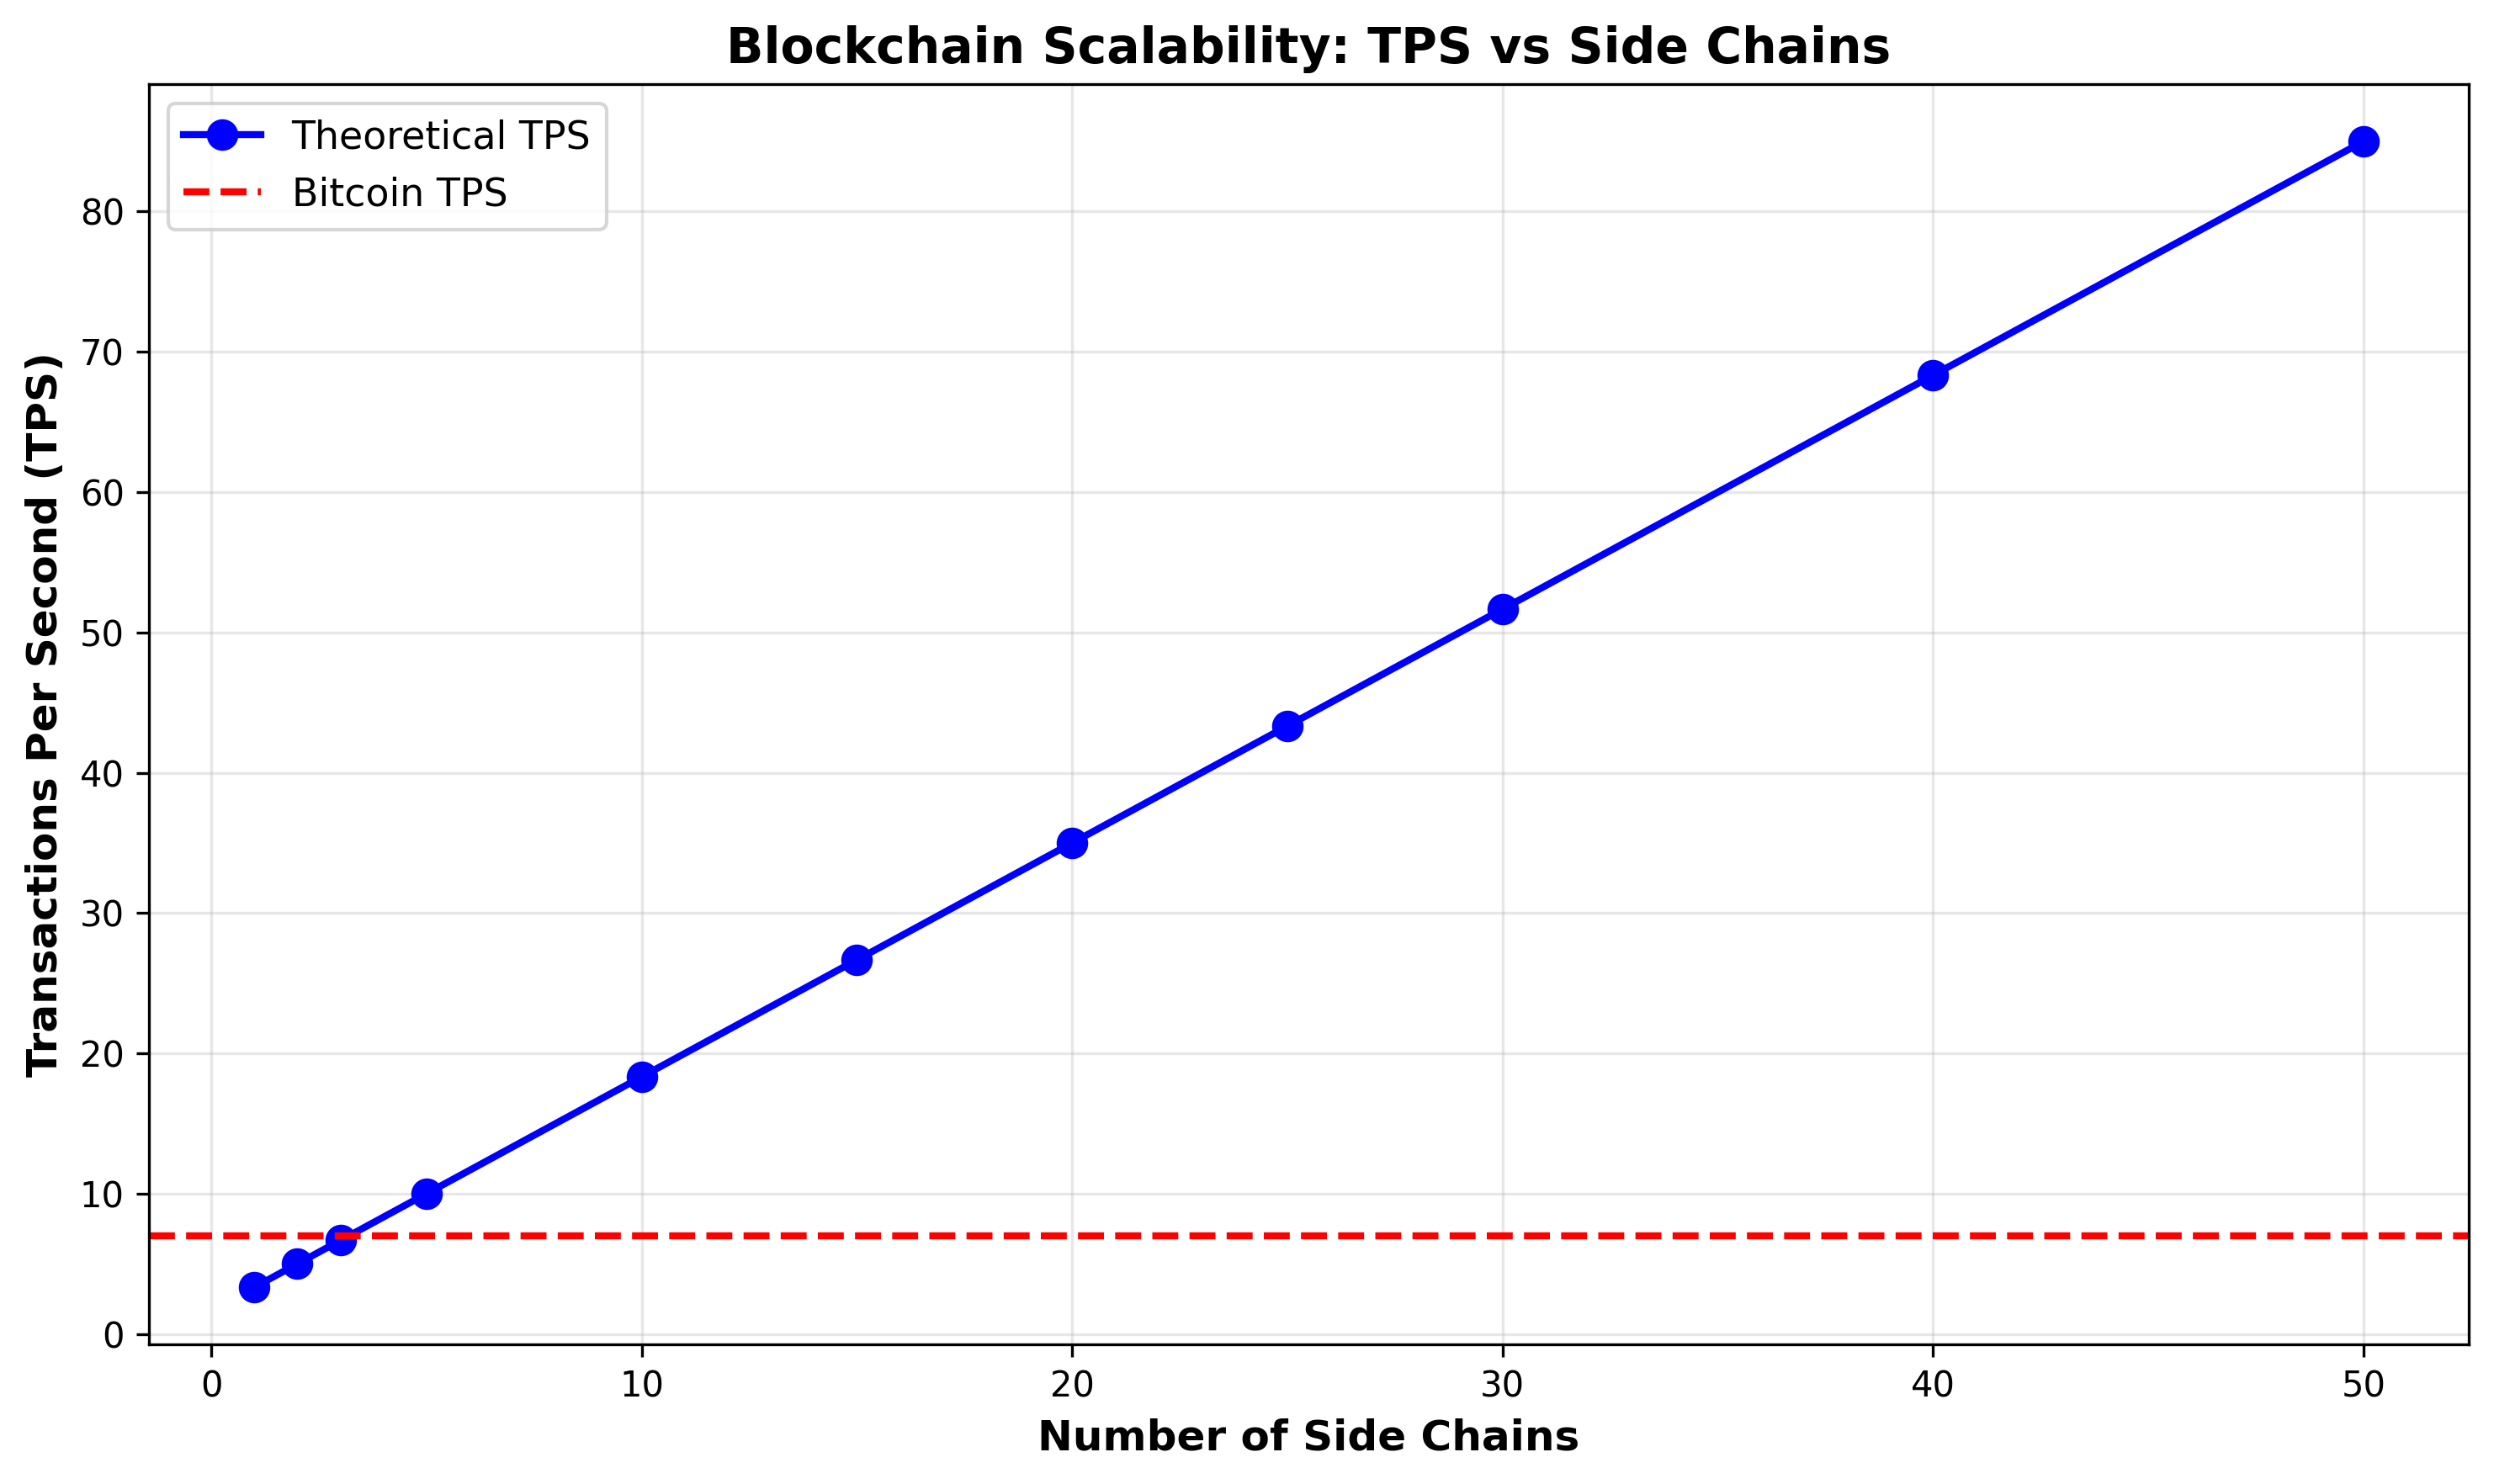
\includegraphics[width=0.88\textwidth,height=0.78\textheight,keepaspectratio]{tps_vs_sidechains.png}
\end{center}

%================ EXPERIMENT ================
\newslide
\slidetitle{محیط آزمایش و روش ارزیابی}
\noindent
\begin{minipage}[t]{0.48\textwidth}
\cardbox{0.92\linewidth}{%
\textbf{\color{UTteal}پارامترهای آزمایش}\\[1mm]
\begin{itemize}
  \item زبان: \lr{Rust} (حالت \lr{Release})
  \item ساختار: \(C_0 + N\) زنجیره جانبی
  \item \(N\) آزمایشی: ۱، ۲، ۳، ۵، ۱۰
  \item دشواری PoW آزمایش: پایین
  \item معیار: میانگین، میانه، min، max، انحراف معیار \lr{TPS}
\end{itemize}}
\end{minipage}\hfill
\begin{minipage}[t]{0.48\textwidth}
\cardbox{0.92\linewidth}{%
\textbf{\color{UTgold}آنچه کامل مدل نشده}\\[1mm]
\begin{itemize}
  \item شبکه \lr{P2P} کامل و تأخیر جغرافیایی
  \item رفتار خصمانه و حملات
  \item هزینه کامل اعتبارسنجی امضا در مقیاس عمومی
  \item اتلاف بسته و رقابت ماینرهای واقعی
\end{itemize}
نتایج = ارزیابی نمونه اولیه، نه بنچمارک تولیدی.}
\end{minipage}

\vspace{4mm}
\keybox{دو دیدگاه ارزیابی جدا نگه داشته شده‌اند: (۱) مدل نظری ظرفیت شبکه بر اساس اندازه/فاصله بلوک؛ (۲) بنچمارک محاسباتی پیاده‌سازی.}

%================ BENCHMARK ================
\newslide
\slidetitle{نتایج بنچمارک محاسباتی (\lr{Rust})}
\begin{center}
\renewcommand{\arraystretch}{1.2}
\begin{tabular}{cccc}
\toprule
\(N\) & تعداد تراکنش آزمون & میانگین TPS & نسبت به \(\approx ۷\) \\
\midrule
۱ & ۵۰ & ۴۴٬۸۲۴٫۸۷ & \(\approx ۶۴۰۴\times\) \\
۲ & ۱۰۰ & ۷٬۶۱۹٫۸۹ & \(\approx ۱۰۸۹\times\) \\
۳ & ۱۵۰ & ۷٬۰۴۹٫۸۴ & \(\approx ۱۰۰۷\times\) \\
۵ & ۲۵۰ & ۱۳٬۷۴۰٫۷۰ & \(\approx ۱۹۶۳\times\) \\
۱۰ & ۵۰۰ & ۸٬۹۳۴٫۴۶ & \(\approx ۱۲۷۶\times\) \\
\bottomrule
\end{tabular}
\end{center}
\vspace{3mm}
\warnbox{\textbf{هشدار روش‌شناختی (مهم برای داوران)}\\[1mm]
این اعداد \textbf{ظرفیت محاسباتی محیط آزمایش} هستند، نه توان عملیاتی شبکه عمومی.\\
دشواری پایین و نبود محدودیت انتشار واقعی، عدد را مصنوعی بزرگ می‌کند.\\
کاهش در برخی پیکربندی‌های چندزنجیره‌ای اثر سربار همزمانی، تعویض زمینه و هماهنگی را نشان می‌دهد.}

%================ FIGURES ================
\newslide
\slidetitle{بهبود نسبت به بیتکوین و مقیاس‌پذیری افقی}
\begin{center}
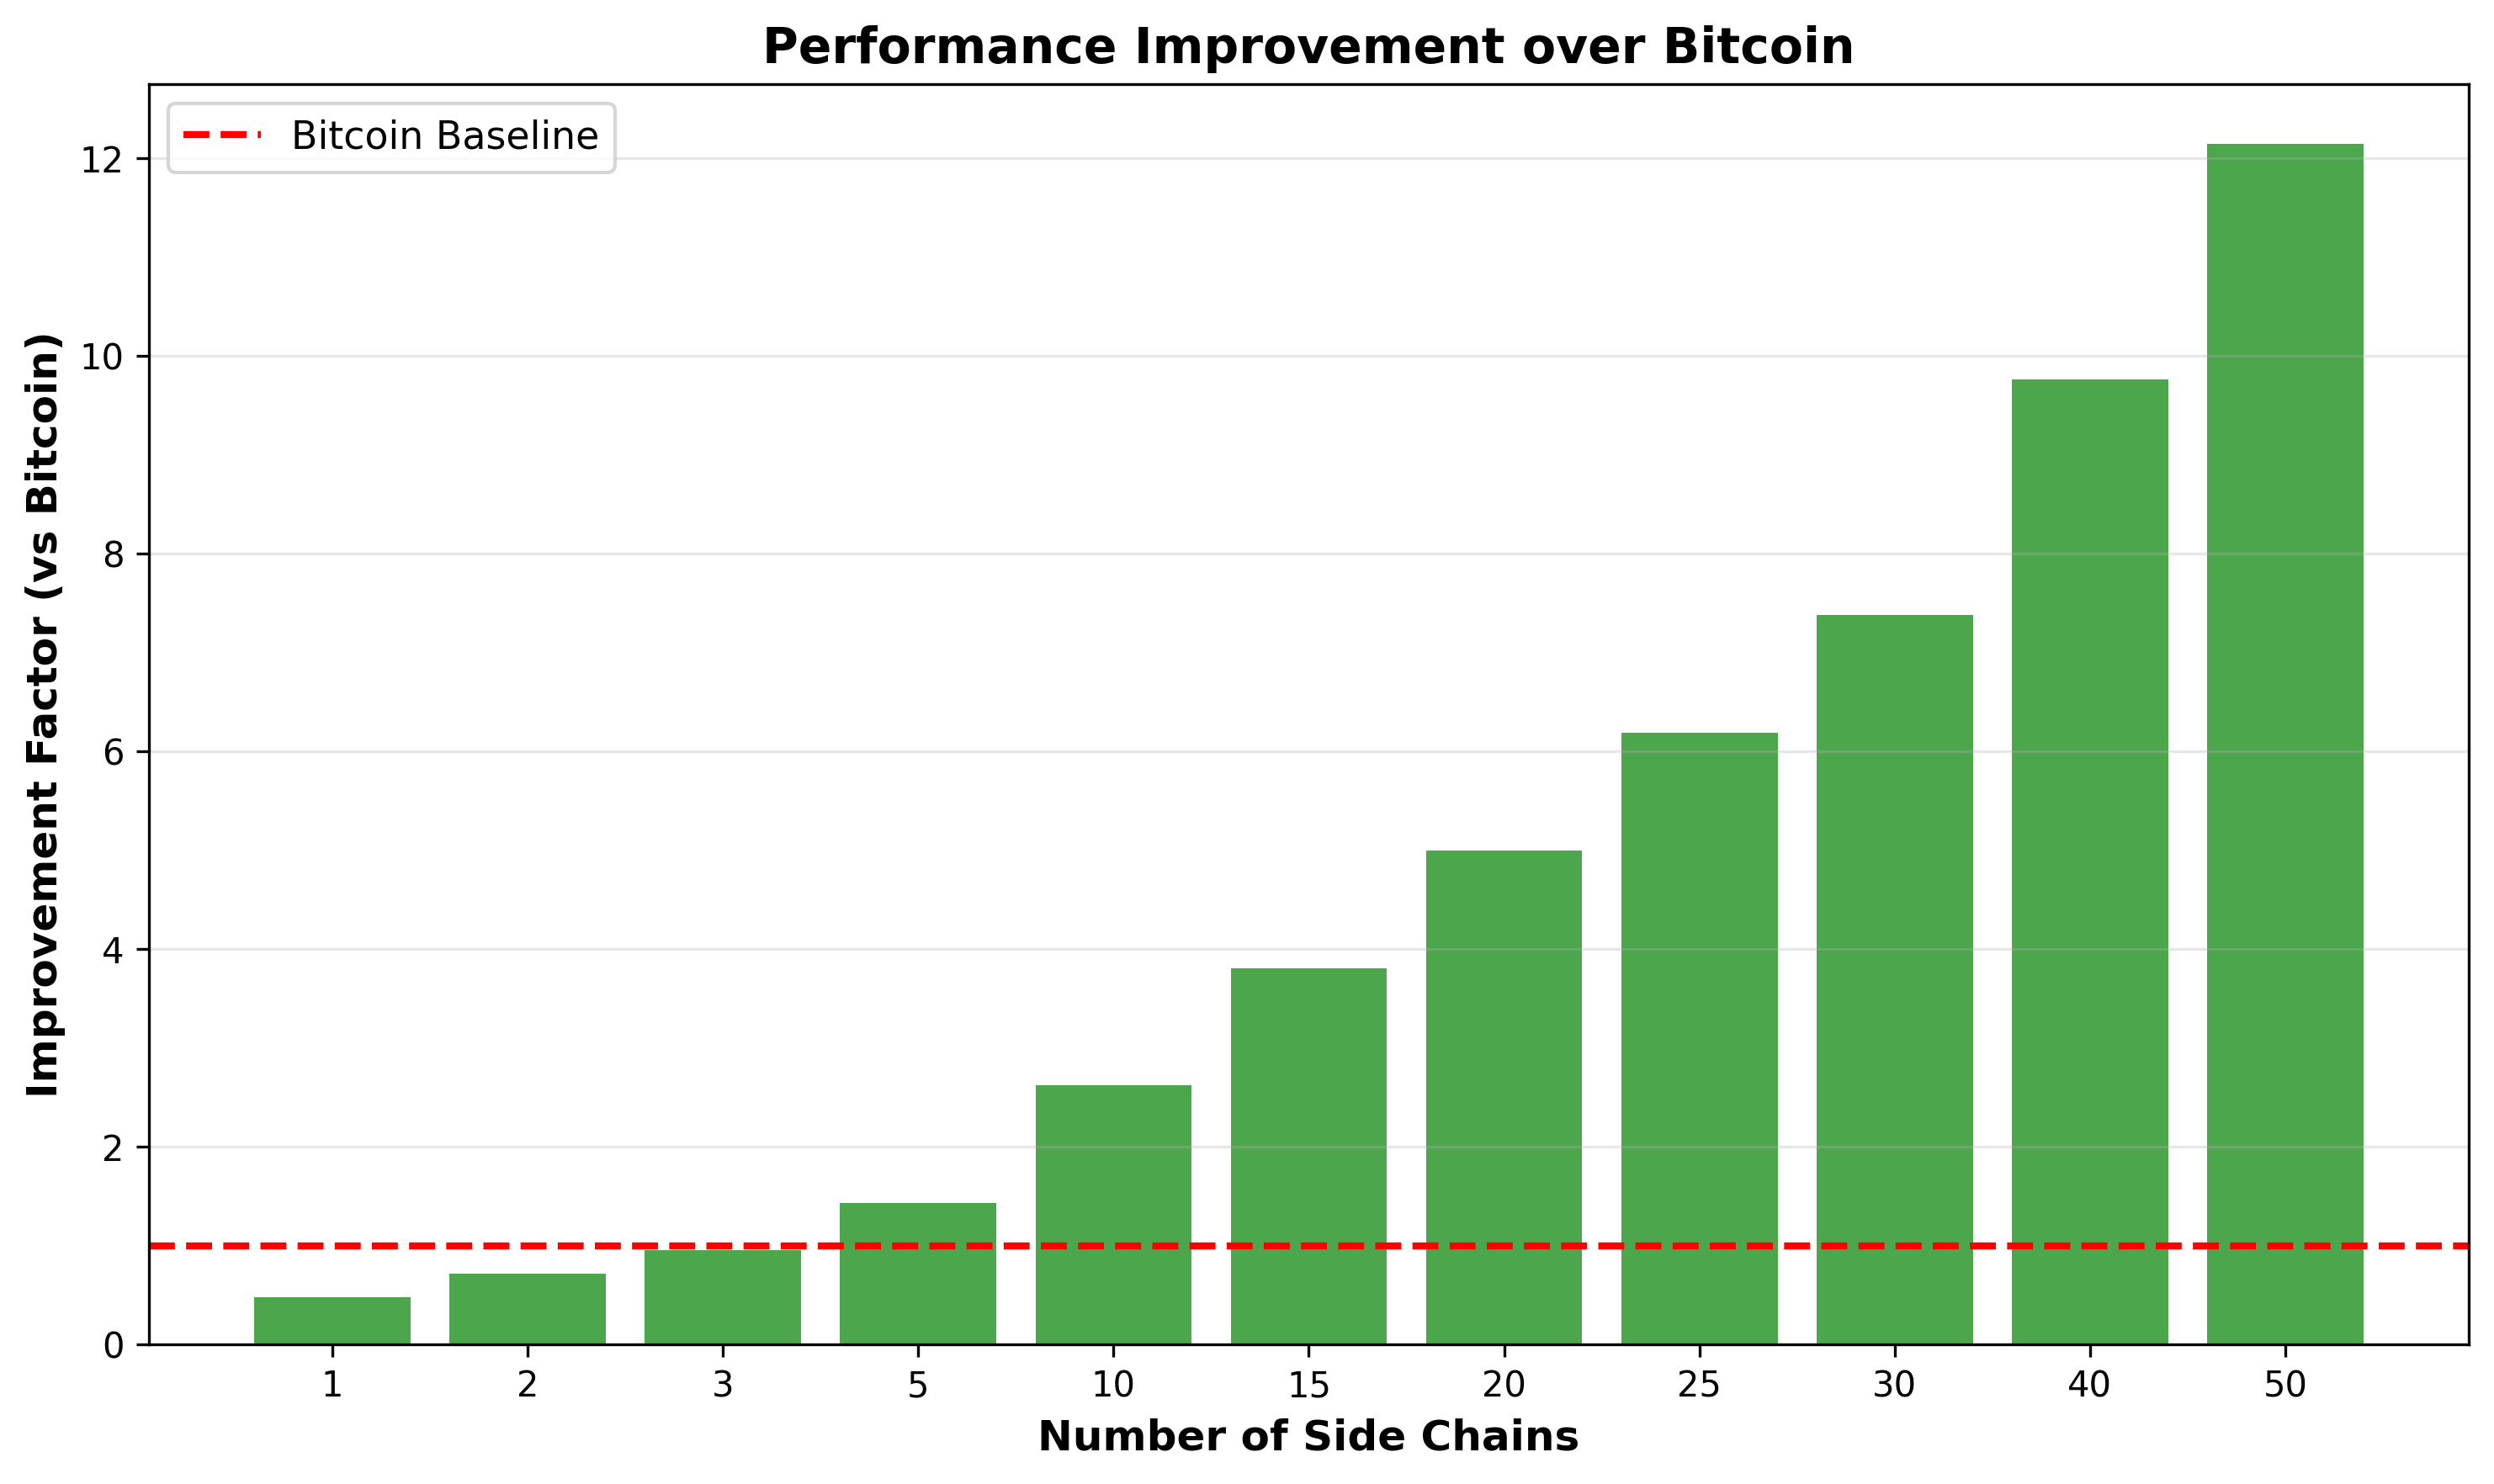
\includegraphics[width=0.48\textwidth,height=0.72\textheight,keepaspectratio]{improvement_vs_bitcoin.png}
\hfill
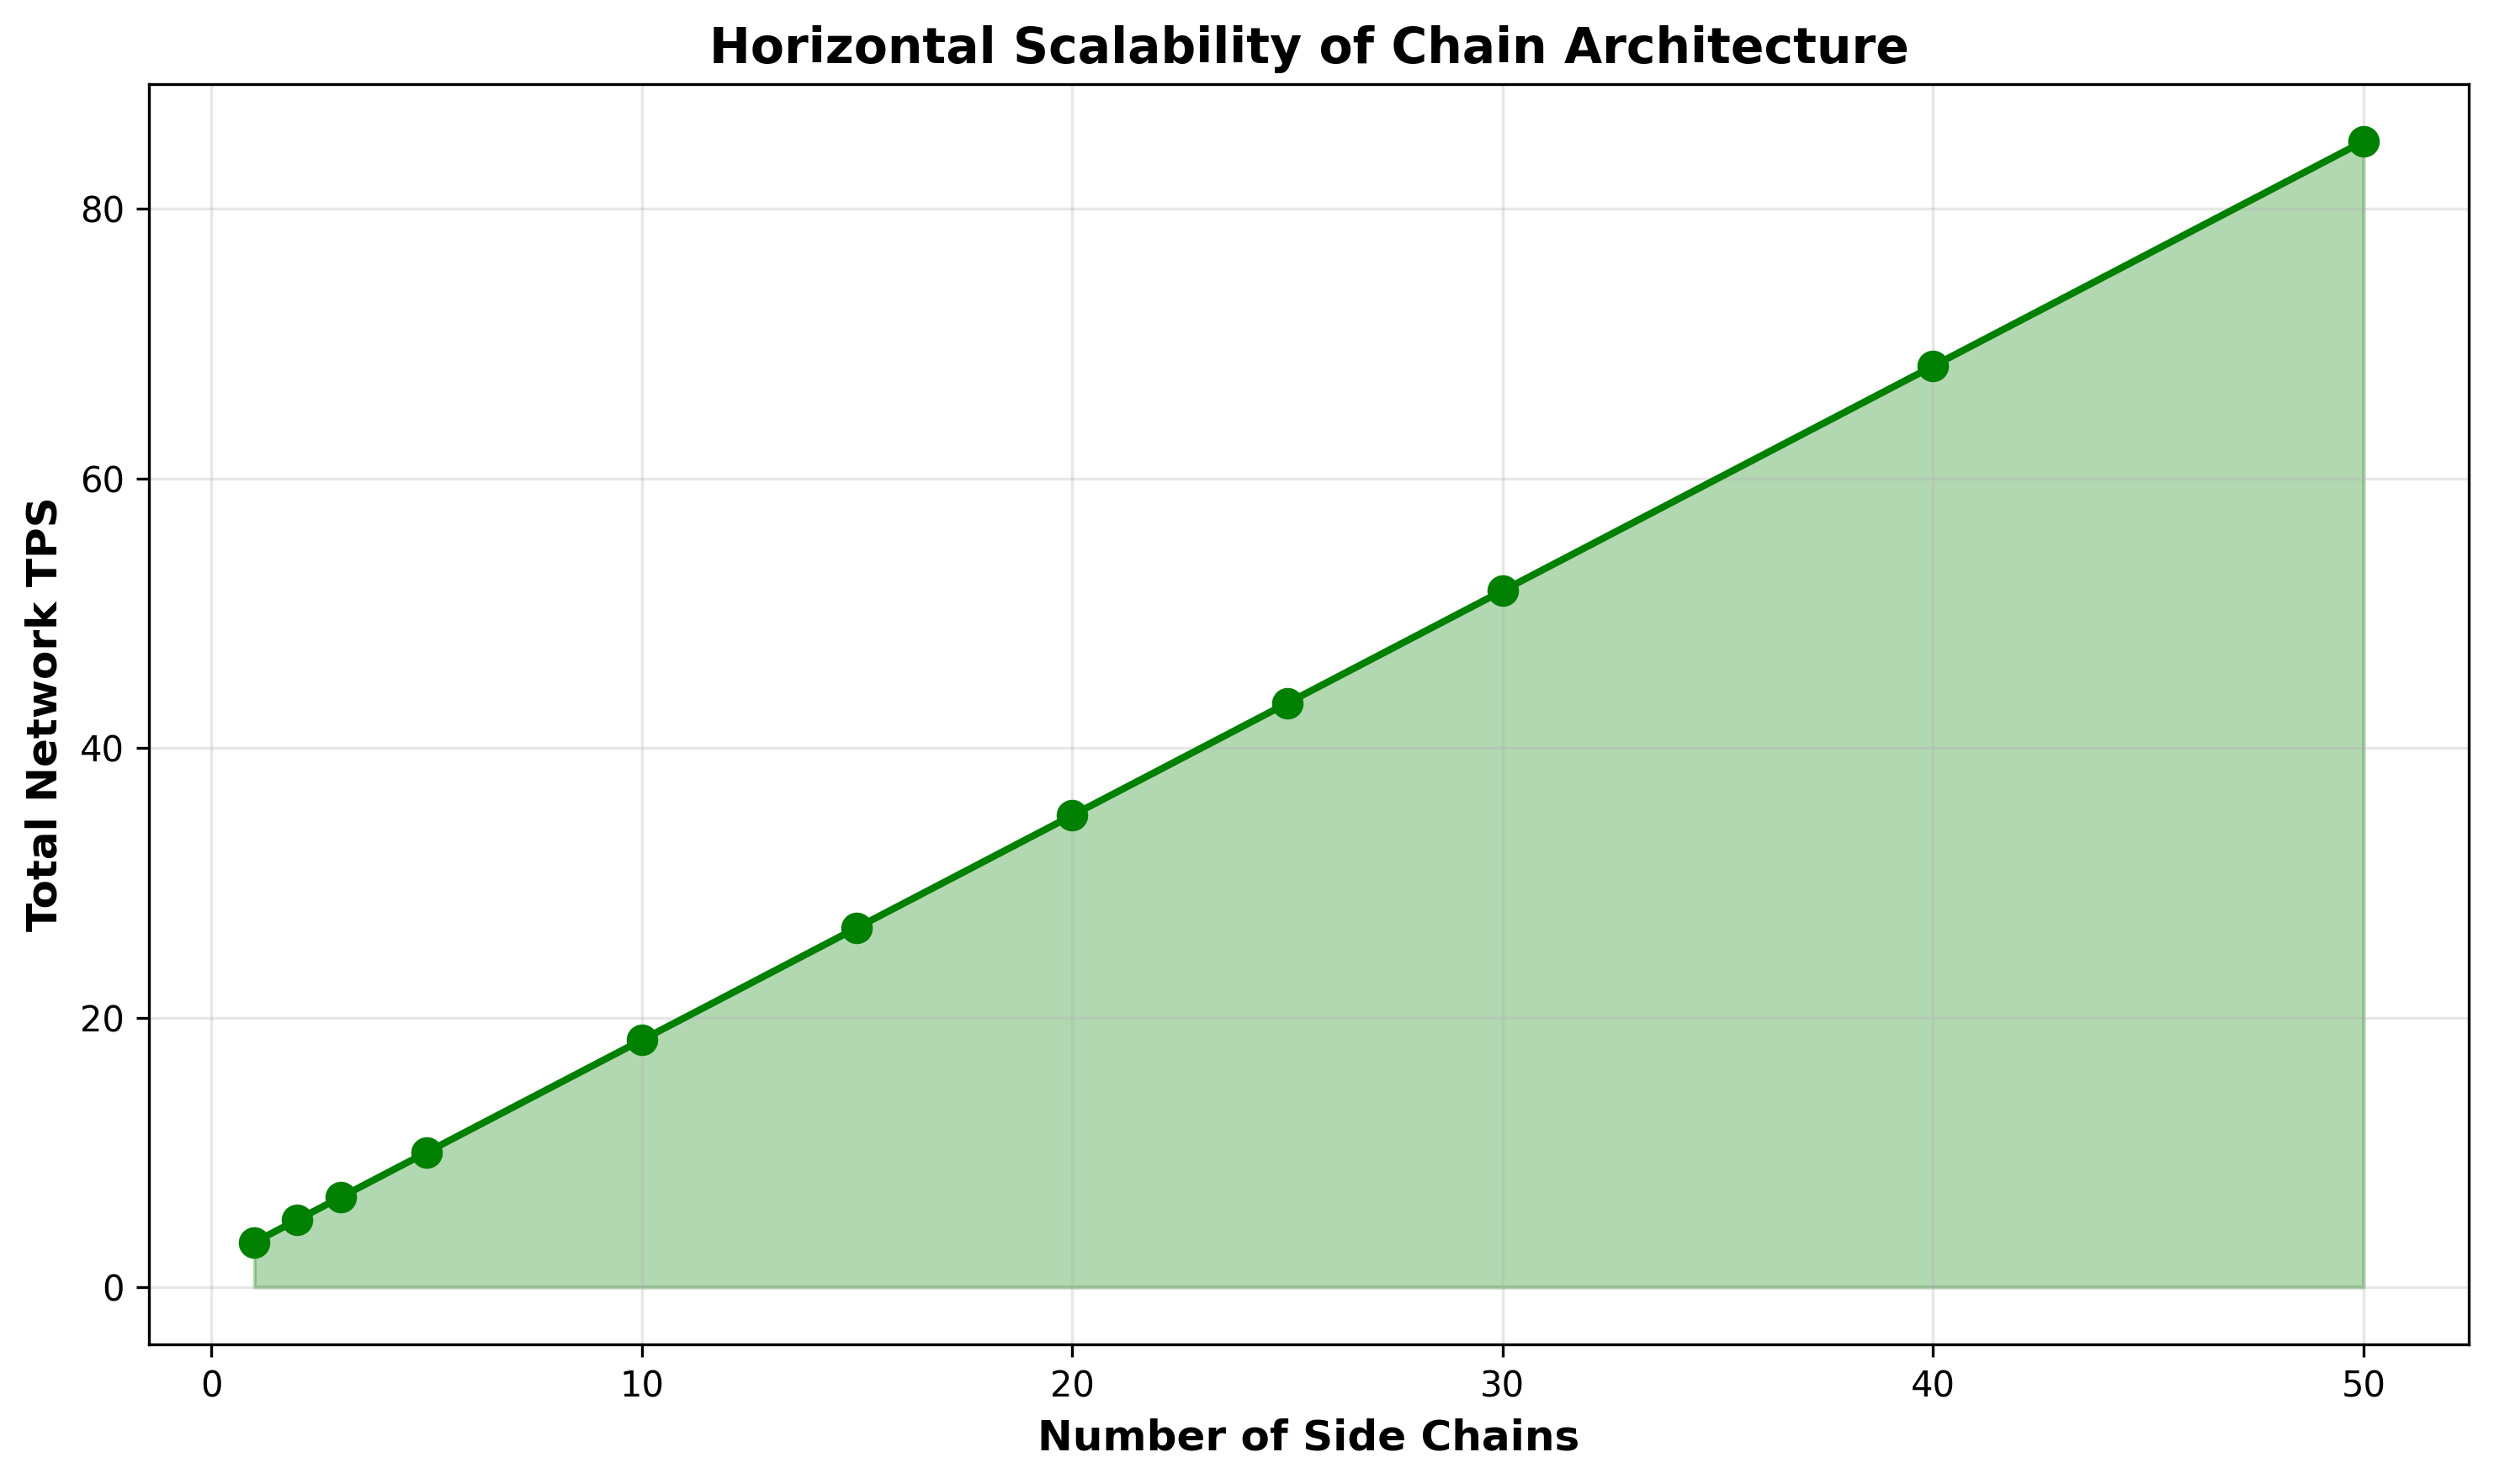
\includegraphics[width=0.48\textwidth,height=0.72\textheight,keepaspectratio]{horizontal_scalability.png}
\end{center}

%================ MAX TPS ================
\newslide
\slidetitle{سقف واقع‌بینانه‌تر و تفاوت دو نوع عدد}
\noindent
\begin{minipage}[t]{0.50\textwidth}
\cardbox{0.92\linewidth}{%
\textbf{\color{UTteal}سقف با محدودیت فیزیکی}\\[1mm]
با بلوک ۱MB، تراکنش \(\approx 0.5\)KB و \(T_s=60\):\\
حدود \(۳۴٫۱۳\) TPS در هر زنجیره.\\[2mm]
با \(N=100\):
\[
TPS_{max}\approx 3.41+3413\approx 3417
\]
معادل حدود \(\mathbf{488\times}\) بیتکوین.}
\end{minipage}\hfill
\begin{minipage}[t]{0.46\textwidth}
\cardbox{0.92\linewidth}{%
\textbf{\color{UTteal}تفکیک دو کمیت}\\[1mm]
\begin{itemize}
  \item \textbf{مدل نظری شبکه:} اندازه و فاصله بلوک
  \item \textbf{بنچمارک:} سرعت پردازش داخلی کد
\end{itemize}
\vspace{1mm}
اشتباه گرفتن این دو با یکدیگر، رایج‌ترین خطای گزارش‌دهی در کارهای مشابه است.}
\end{minipage}
\vspace{3mm}
\begin{center}
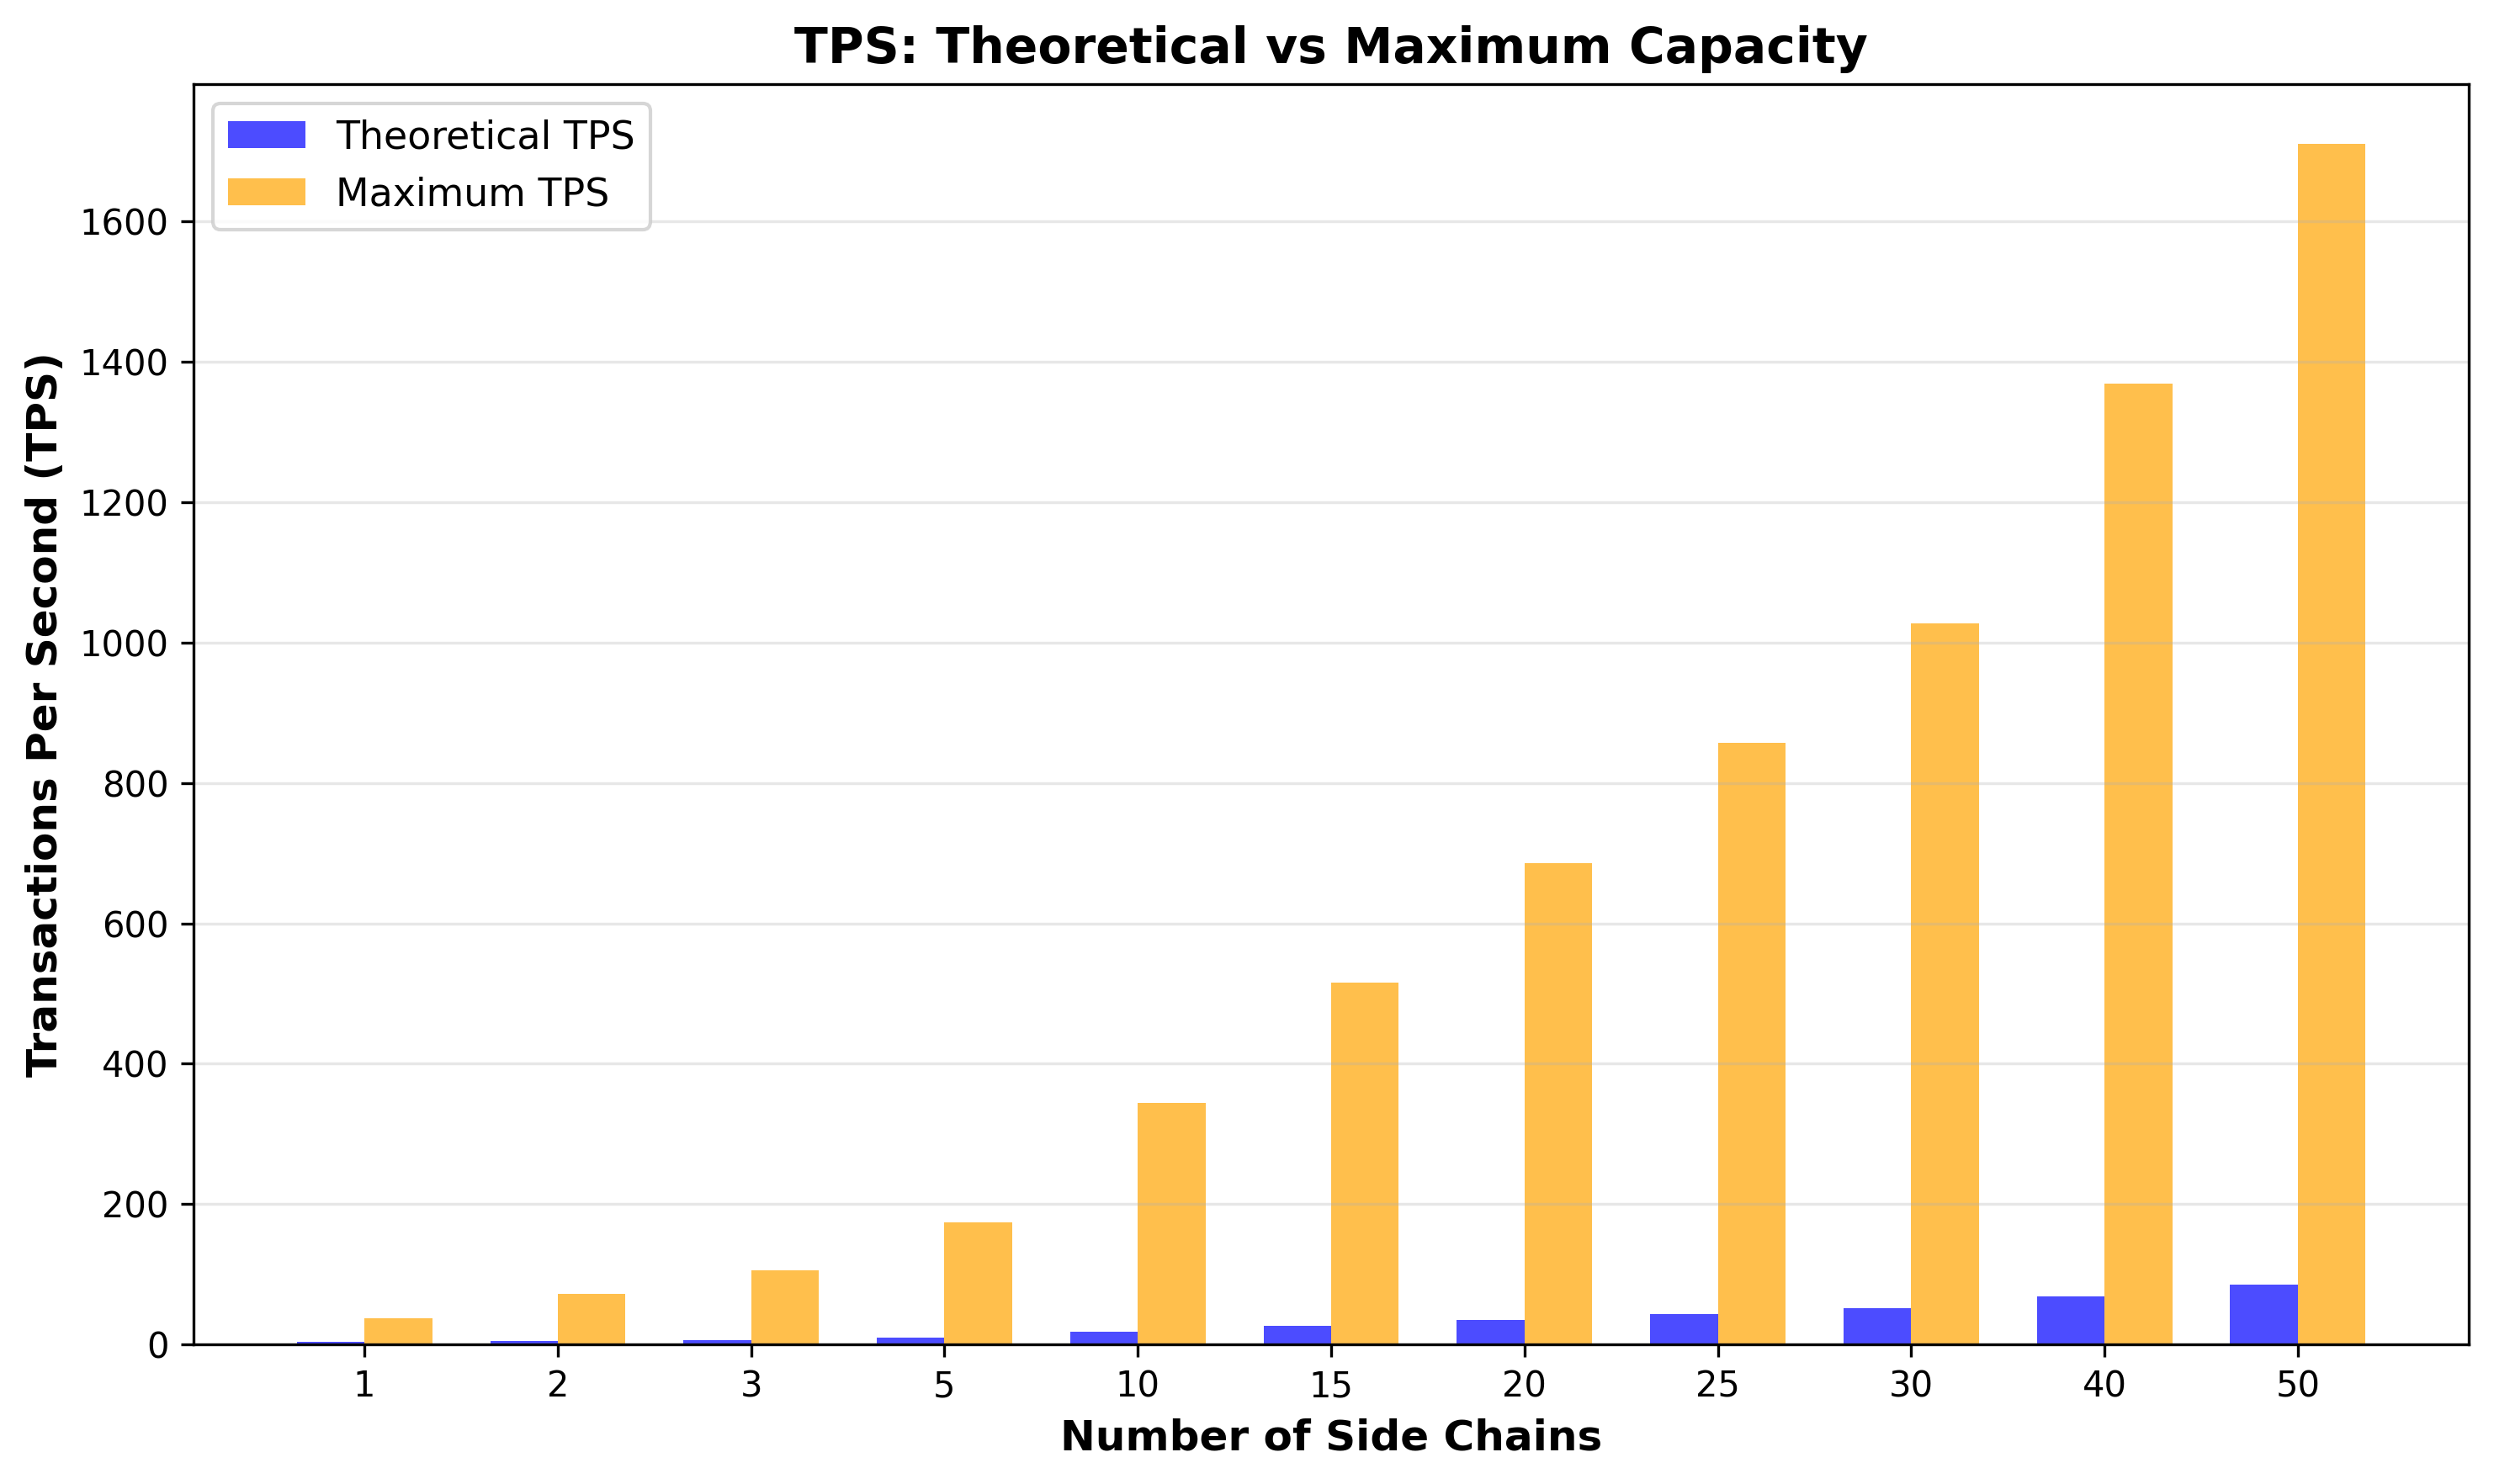
\includegraphics[width=0.70\textwidth,height=0.38\textheight,keepaspectratio]{tps_theoretical_vs_max.png}
\end{center}

%================ VALIDITY ================
\newslide
\slidetitle{تهدیدهای اعتبار ارزیابی}
\begin{itemize}
  \item \textbf{اعتبار داخلی:} نمونه کوچک تراکنش‌ها، دشواری پایین یا ساختار داده ساده می‌تواند عدد را مصنوعی بالا ببرد.
  \item \textbf{اعتبار خارجی:} نتایج یک محیط آزمایشی لزوماً به شبکه جهانی با هزاران نود تعمیم‌پذیر نیست.
  \item \textbf{اعتبار سازه‌ای:} فقط \lr{TPS} کافی نیست؛ تأخیر، قطعیت نهایی، نرخ فورک و هزینه نود نیز باید بررسی شوند.
  \item \textbf{اعتبار بازتولید:} نسخه کد، سخت‌افزار، سیستم‌عامل، پارامترها و روش اجرا باید ثبت شوند.
\end{itemize}
\vspace{3mm}
\keybox{\textbf{سهم روش‌شناختی:} شفافیت گزارش‌دهی بخشی از سهم پژوهش است. عددهای بزرگ بدون زمینه قابل دفاع نیستند؛ تفکیک بنچمارک از ظرفیت شبکه، ادعا را قابل بازتولید نگه می‌دارد.}

%================ SECURITY ================
\newslide
\slidetitle{تحلیل امنیت (خلاصه)}
\noindent
\begin{minipage}[t]{0.48\textwidth}
\cardbox{0.92\linewidth}{%
\textbf{\color{UTteal}زنجیره اصلی}\\[1mm]
PoW با دشواری بالاتر؛ کار انباشته؛ مرجع نهایی فورک و بازسازماندهی؛ مرجع قطعیت اقتصادی.}
\vspace{2mm}
\cardbox{0.92\linewidth}{%
\textbf{\color{UTteal}تخصیص}\\[1mm]
قطعی، عمومی، بدون هماهنگ‌کننده؛ هر خروجی یک قلمرو → محدودسازی سطح حمله دوبارخرج.}
\end{minipage}\hfill
\begin{minipage}[t]{0.48\textwidth}
\cardbox{0.92\linewidth}{%
\textbf{\color{UTteal}زنجیره جانبی}\\[1mm]
قلمرو محدود \lr{UTXO}؛ ارجاع دوره‌ای به اصلی؛ تأیید اولیه \(\neq\) قطعیت نهایی.}
\vspace{2mm}
\cardbox{0.92\linewidth}{%
\textbf{\color{UTgold}بین‌زنجیره‌ای}\\[1mm]
نیاز به قفل اتمیک + اثبات مرکل + مهلت/بازگردانی.\\
در نسخه اولیه نیازمند تکمیل و اثبات امنیتی دقیق‌تر است.}
\end{minipage}

%================ ANSWERS ================
\newslide
\slidetitle{پاسخ کوتاه به پرسش‌های پژوهش}
\begin{enumerate}
  \item \textbf{تقسیم بدون دوبارخرج:} تخصیص مبتنی بر هش \lr{UTXO}؛ هر خروجی فقط در یک قلمرو خرج می‌شود.
  \item \textbf{نقش \(C_0\):} نه محل همه تراکنش‌ها، بلکه مرجع امنیتی، زمان‌سنج و مرجع نهایی ارجاعات.
  \item \textbf{رابطه با \(N\):} تحت فرض تقارن، رشد تقریباً خطی \(TPS\approx 6.99+69.90N\).
  \item \textbf{نظری در برابر بنچمارک:} اولی محدودیت بلوک/شبکه؛ دومی سقف پردازشی نرم‌افزار آزمایشگاهی.
  \item \textbf{ریسک‌ها:} امنیت جانبی، بین‌زنجیره‌ای، داده‌دسترسی، هماهنگی، عدم تعادل بار.
\end{enumerate}

%================ CONTRIBUTIONS ================
\newslide
\slidetitle{دستاوردها و محدودیت‌ها}
\noindent
\begin{minipage}[t]{0.48\textwidth}
\cardbox{0.92\linewidth}{%
\textbf{\color{UTteal}دستاوردهای اصلی}\\[1mm]
\begin{itemize}
  \item تکسونومی تحلیلی روش‌های مقیاس‌پذیری
  \item معماری Master + Side Chains
  \item تابع تخصیص قطعی مبتنی بر \lr{UTXO}
  \item مدل ریاضی رشد خطی ظرفیت
  \item پیاده‌سازی نمونه اولیه \lr{Rust} (متن‌باز)
  \item تفکیک صریح بنچمارک از ظرفیت شبکه
  \item شناسایی ریسک‌های امنیتی و مهندسی
\end{itemize}}
\end{minipage}\hfill
\begin{minipage}[t]{0.48\textwidth}
\cardbox{0.92\linewidth}{%
\textbf{\color{UTgold}محدودیت‌ها}\\[1mm]
\begin{itemize}
  \item نمونه اولیه \(\neq\) شبکه تولیدی کامل
  \item پروتکل بین‌زنجیره‌ای نیازمند تکمیل
  \item امنیت جانبی با دشواری پایین‌تر
  \item داده‌دسترسی نیازمند طراحی دقیق‌تر
  \item بنچمارک وابسته به سخت‌افزار آزمایش
  \item شبیه‌سازی تأخیر شبکه کامل نشده
\end{itemize}}
\end{minipage}

%================ FUTURE ================
\newslide
\slidetitle{کارهای آینده}
\begin{enumerate}
  \item طراحی و پیاده‌سازی پروتکل کامل بین‌زنجیره‌ای با قفل اتمیک و اثبات مرکل
  \item بررسی استخراج ادغام‌شده (\lr{Merged Mining}) برای افزایش امنیت زنجیره‌های جانبی
  \item سیاست دوره‌بندی (\lr{Epoch}) برای تغییر تعداد زنجیره‌ها بدون جابه‌جایی ناگهانی تخصیص
  \item افزودن داده‌دسترسی و نمونه‌برداری داده برای بلوک‌های جانبی
  \item بنچمارک توزیع‌شده روی چند ماشین با شبیه‌سازی تأخیر شبکه
  \item تحلیل اقتصادی کارمزدها، پاداش ماینرها و انگیزه مشارکت
  \item مقایسه تجربی کنترل‌شده با شاردینگ، رول‌آپ و زنجیره جانبی کلاسیک
  \item وارسی رسمی (\lr{Formal Verification}) پروتکل نهایی‌سازی و بین‌زنجیره‌ای
\end{enumerate}

%================ CONCLUSION ================
\newslide
\slidetitle{نتیجه‌گیری}
\keybox{\textbf{پیام اصلی}\\[1mm]
با جداسازی نقش \textbf{امنیت} و \textbf{پردازش} می‌توان ظرفیت بالاتر از معماری تک‌زنجیره‌ای داشت و همچنان از زنجیره اصلی اثبات کار برای قطعیت نهایی استفاده کرد.}
\vspace{3mm}
\begin{itemize}
  \item مقیاس‌پذیری افقی: افزودن زنجیره جانبی ≈ افزودن سهم ثابت به \(TPS\)
  \item امنیت نهایی به \(C_0\) گره می‌خورد؛ تأیید اولیه سریع‌تر روی زنجیره‌های جانبی است
  \item عددهای عملکردی بدون زمینه (شبکه در برابر آزمایشگاه) قابل دفاع نیستند
  \item این معماری جایگزین همه راهکارها نیست؛ چارچوبی قابل تحلیل برای ترکیب PoW، زنجیره جانبی و پردازش موازی است
\end{itemize}
\vspace{2mm}
\warnbox{\textbf{جمله پایانی:} مقیاس‌پذیری واقعی نه از یک ترفند منفرد، بلکه از طراحی دقیق رابطه میان اجماع، داده، اعتبارسنجی، امنیت و تجربه کاربری حاصل می‌شود.}

%================ THANKS ================
\newslide
\thispagestyle{empty}
\begin{tikzpicture}[remember picture,overlay]
  \fill[UTnavy] (current page.south west) rectangle (current page.north east);
  \fill[UTgold] ([yshift=-62mm]current page.north west) rectangle ([yshift=-63.2mm]current page.north east);
\end{tikzpicture}
\vspace*{28mm}
\begin{center}
{\Huge\textbf{\textcolor{white}{با سپاس از توجه شما}}}\\[8mm]
{\LARGE\textcolor{UTgold}{آماده پاسخگویی به پرسش‌های اساتید محترم}}\\[14mm]
{\large\textcolor{UTsoft}{سجاد خشدونی فراهانی}}\\[2mm]
{\normalsize\textcolor{UTsoft}{استاد راهنما: دکتر علی کمندی}}\\[1mm]
{\normalsize\textcolor{UTsoft}{دانشگاه تهران — دانشکده علوم مهندسی}}\\[8mm]
{\small\textcolor{UTsoft}{کلیدواژه‌ها: بلاکچین، مقیاس‌پذیری، زنجیره اصلی، زنجیره جانبی، اثبات کار، \lr{TPS}}}
\end{center}

\end{document}
